\documentclass[12pt]{article}
\usepackage{url}
\usepackage{setspace}
\usepackage[superscript]{cite}
\usepackage{graphicx}
\usepackage[normalem]{ulem}
\graphicspath{ {Figures/} }
\usepackage{caption}
\usepackage{cite}
\usepackage{indentfirst}
\usepackage{float}
\usepackage{subcaption}
\usepackage{amsmath}
\textwidth=6.5in
\oddsidemargin=0.0in
\usepackage{listings}
\usepackage{listings}
\usepackage{fancyhdr}
\usepackage{longtable}
\usepackage[table]{xcolor}
\pagestyle{fancy}
\fancyhf{}
\lhead{Personal Study Assistant}
\rhead{Page \thepage}

\usepackage{color}
\usepackage{hyperref}
\hypersetup{
    colorlinks=true,
    citecolor=black,
    linktoc=all,
    linkcolor=black,
}

\begin{document}

\begin{titlepage}

    \newcommand{\HRule}{\rule{\linewidth}{0.5mm}}

    \center

    \textsc{\LARGE Missouri State University\\~\\Department computer Science}\\[1.0cm]

    \HRule \\[0.4cm]
    { \huge \bfseries Personal Study Assistant}\\[0.4cm]
    \HRule \\[1.5cm]


    \begin{minipage}{0.4\textwidth}
        \begin{flushleft} \large
            Trey Alexander \\
            Mackensie Bass \\
            Ali Karimiafshar \\
            Anh Minh Nhat Doan \\
            Bryan Leach \\
        \end{flushleft}
    \end{minipage}
    ~
    \begin{minipage}{0.4\textwidth}
        \begin{flushright} \large
            Dr. Belkouche \\
            YassineBelkhouche@missouristate.edu
        \end{flushright}
    \end{minipage}\\[2cm]

    {\large \today}\\[2cm]

\end{titlepage}

\newpage
%-----------------------------------------------------------------------
\tableofcontents

\newpage
%----------------------------------------------------------------------

%-----------------------------------------------------------------------------
\section{Project description}
\subsection{Description}
Google Chrome Extension to help students study by minimizing distractions from other websites.
This is inspired by The Pomodoro Technique which recommendes studying for 25 minutes, then a 5 minute break, repeating that 3 times and then having a longer break.
During study time, the user will only be allowed to access approved websites such as Google Classroom. This will be handled through a whitelist of approved websites.
During the break time, the user is allowed to access any website they desire, but they are encouraged to practice healthy activites like stretching or drinking water.
The user's keyboard and mouse inputs will be monitored to measure if they are actively working.
% \subsection{Key Components}
% \begin{itemize}
%     \item Timer that switches between study time and break time
%     \item Whitelist of a pproved websites
%     \item Parental controls to alter the whitelist
%     \item Record of past sessions and the all time totals for study time
% \end{itemize}
% \subsection{Knowledge Required for Developers}
% \begin{itemize}
%     \item HTML
%     \item CSS
%     \item JavaScript
%     \item How to make Chrome Extension
%     \item Locally host a webpage
% \end{itemize}
% \subsection{Hardware required for the user}
% \begin{itemize}
%     \item Computer
%     \item Internet
%     \item Google Chrome Browser
% \end{itemize}

\section{Requirements Specification}
\subsection{Functional Requirements}
\begin{itemize} %this is to fix the tab that is being added automatically
\end{itemize}
Req-01: On the first run, get information from the user.
\begin{itemize}
    \item Description: The function makes the user provide their chosen username and a parent pin. 
    \item Rationale: Student provides information to personalize the experience. Parent pin allows for access to control the whitelist.
    \item Input(s): Input information about the user and the chosen parent pin.
    \item Output(s): N/A.
    \item Dependency: N/A.
\end{itemize}
Req-02: Users can choose from a list of timer options when the extension is started.
\begin{itemize}
    \item Description: The function lets users choose from a list of timer options. Example options would be A- 25 min study, 5-minute break, 3 times, 15 min long break or B- 45 minute study, 10 minute break, 3 times, 30 minute long break.
    \item Rationale: User might want to study for different amounts of time different days so this lets them choose.
    \item Input(s): Function receive option result from users.
    \item Output(s): Begin chosen session type.
    \item Dependency: N/A.
\end{itemize}
Req-03:  There is a Timer to keep track of study and break time.
\begin{itemize}
    \item Description: A timer is running to keep track of users’ study time and break time. Timer can be paused, resumed, and reset by the user and system. Change color in study mode and break mode. Can be hidden or unhidden by the user.
    \item Rationale: It is easy to loose track of time or think that a lot more time has passed than really did while studying. A timer allows the user to know exactly how long they have been working, and how much longer they have.
    \item Input(s): Amount of time to start at, values for pause , resume, and hide the timer.
    \item Output(s): Send an alert when timer reaches 00:00. 
    \item Dependency: Timer amount from Req-02.
\end{itemize}
Req-04: Keyboard and mouse interactions are monitored to detect if the user has stopped working.
\begin{itemize}
    \item Description: User's keyboard and mouse inputs are monitored on an occurrence basis to ensure the user has not stopped working while not recording the contents of such inputs for privacy.
    \item Rationale: If a specified period of time elapses with no input from the user detected, it is likely the user has stopped working and measures must be take to help the user stay focused.
    \item Input(s): Mouse clicks and movements, as well as keyboard keystrokes.
    \item Output(s): Req-05 is called.
    \item Dependency: N/A.
\end{itemize}
Req-05: If no user inputs detected according to Req-04 after a predetermined amount of time, alert the user with a prompt to verify they are still working.
\begin{itemize}
    \item Description: When the conditions of Req-04 are met, the user is prompted to verify they are still working. The study timer is paused until the user verification is complete.
    \item Rationale: Asking for user interaction to verify they are still working encourages more engagement with the material and ensures the user is present and attentive during the study times.
    \item Input(s): Req-04.
    \item Output(s): Prompt to user in the form of a pop up, or other contents.
    \item Dependency: Req-04.
\end{itemize}
Req-06: During study time, check if the Google Chrome browser is in focus.
\begin{itemize}
    \item Description: The function checks if the browser window is in focus every few seconds. If it is found not to be, then the value is changed to false.
    \item Rationale: If the Google Chrome browser window is not in focus during study time, then the user is not studying so the extension needs to get them back on task.
    \item Input(s): N/A.
    \item Output(s): The in-focus value is changed to false, and Req-07 is called.
    \item Dependency: N/A.
\end{itemize}
Req-07: During study time, send an alarm and alert to the user if the Google Chrome browser is not in focus, and pause the timer.
\begin{itemize}
    \item Description: During study time, an alarm will sound when the extension detects the Google Chrome browser is not the in-focus window. When the user comes back to the page, an alert will show explaining the alarm sounded because the browser window was out of focus.
    \item Rationale: The purpose of the alarm and alert is to try to prevent the user from using other applications on the computer when they should be studying. The extension cannot prevent other applications, but it can encourage the user to stay on task.
    \item Input(s): Function receives a value of false.
    \item Output(s): Sends out an alert and alarm to the user and pauses the timer until the alarm and alert is stopped.
    \item Dependency: Gets input from Req-06, access timer through Req-03.
\end{itemize}
Req-08: Implement a whitelist for only previously approved websites.
\begin{itemize}
    \item Description: During study time, the user is only allowed to visit previously approved websites as specified in the whitelist.
    \item Rationale: If the user is allowed to access non-educational sites such as social media or games, then they will not be focused on studying and will be wasting time. 
    \item Input(s): Can accept new additions to the whitelist from the user’s parental figure with their pin.
    \item Output(s): N/A.
    \item Dependency: May receive input from Req-09 if a new site is added.
\end{itemize}
Req-09: During study time, access to a non-approved site will result in access to the site being blocked. Option to add the site to the whitelist is displayed with the alert.
\begin{itemize}
    \item Description: Access to a site not on the whitelist will be blocked and a message will show explaining that it has been blocked. An option to add the site to the whitelist will also show but will require a parent pin to add it.
    \item Rationale: Sites not on the approved whitelist should be blocked when attempted to access because the user will not be studying if they are trying to access social media. But, if the site is a new educational resource, then the parent should be able to add it to the list of approved sites. 
    \item Input(s): The whitelist so that the function can see if a site is not allowed.
    \item Output(s): Block the site, send an alert, add a new website to whitelist if they choose to do so.
    \item Dependency: Receives the whitelist form Req-08.
\end{itemize}
Req-10: When study time ends, display a message for the user to choose to begin or postpone the break.
\begin{itemize}
    \item Description: When the study time ends, congratulate the user, and ask if they are ready for their break by displaying a “Start Break” button, and a “Postpone for x minutes” button with a drop-down menu selector for 1, 2, 3, 4, or 5 minutes more. Function will call the short or long break depending on the value of numOfShortBreaksLeft.
    \item Rationale: The user must take short breaks to avoid burn out which would result in less effective studying.
    \item Input(s): Called when the study timer ends.
    \item Output(s): Send the message to the user to being or postpone the break.
    \item Dependency: Receives the end timer message from Req-03.
\end{itemize}
Req-11: Short break: If a break is started, decrease the number of short breaks needed until a long break and begin break time.
\begin{itemize}
    \item Description: During break time, the user is allowed to visit non-approved sites and can change the window. There will be a message shown when break time starts to encourage the user to participate in healthy activities such as drinking water, having a healthy snack, and doing some stretches.  This function will also update numOfShortBreaksLeft that decides how many more short breaks there must be until a long break.
    \item Rationale: The Pomodoro Technique says to have short breaks for a few cycles, then a long break before starting again to help prevent burn out and to use time wisely. The users should be allowed to do whatever they would like during break time, but the pomodoro technique recommends healthy activities and not scrolling social media.
    \item Input(s): N/A.
    \item Output(s): Timer is changed to count down until the break is over.
    \item Dependency: Access the user’s input from Req-10 and access the timer from Req-03.
\end{itemize}
Req-12: Long break: If it is time for a long break, begin the break.
\begin{itemize}
    \item Description: This function begins the long break which happens once per session after a few cycles of study time and short breaks.
    \item Rationale: The Pomodoro Technique recommends having a long break after having a few short breaks.
    \item Input(s): N/A.
    \item Output(s): Break message is sent out like the message for short break from Req-11.
    \item Dependency: Is called from Req-10 and accesses the timer from Req-03.
\end{itemize}
Req-13: If the break is postponed, turn timer red and keep counting.
\begin{itemize}
    \item Description: This function activates when the user does not take the prompted break. Turning the timer read and continuing to count.
    \item Rationale: Lets the user know that they need to take their break and that the timer is still counting.
    \item Input(s): User not having hit the break button.
    \item Output(s): Continues counting, but font is now red.
    \item Dependency: Input from Req-10 and timer from req-03.
\end{itemize}
Req-14: Do not allow for the study tabs to be opened during the break time
\begin{itemize}
    \item Description: Does not allow the user to open the tabs they were using for studying during the break.
    \item Rationale: Forces the user to actually take their break.
    \item Input(s): Study timer and break timer.
    \item Output(s): Lock / unlock
    \item Dependency: Input from Req-10 and timer from Req-03.
\end{itemize}
Req-15: At the end of the break, display an alert to begin the next session, and play an audio alert if no response for 1 minute. If this is the end of a long break, ask if they want to restart the same session, stop, or choose a different session
\begin{itemize}
    \item Description:  Asks user at the end of their break if they would like to begin their session again and ask if they want to resume, stop, or start a new session. Plays an audio alert after a minute if no response.
    \item Rationale: Allows user to decide their next steps after a break.
    \item Input(s): User says: resume, stop, start new. 
    \item Output(s): Repeats user’s input and reacts with the appropriate action. Resumes where user left off, stops the program, or starts a new session.
    \item Dependency:  Input from Req-10 and timer from Req-03.
\end{itemize}
Req-16: Allow parents to approve new websites with a parent pin
\begin{itemize}
    \item Description: Allows access to new websites with parent’s approval via a chosen PIN.
    \item Rationale: User can only visit approved sites during study sessions.
    \item Input(s): Parent PIN, website URL.
    \item Output(s): User can now visit that website during study sessions.
    \item Dependency: Req-09 to bring up whitelist option.
\end{itemize}
Req-17: Website for user to view their history, progress data, statistics, and reports, as well as participate in gamification.
\begin{itemize}
    \item Description: The user will have the option to log into a website (available on localhost for this project's scope; this website could be deployed on a specific domain) where useful data about their progress can be viewed. The user will be able to participate in gamification to encourage improvements over time.
    \item Rationale: A centralized location for the user to view all of their data can be very useful to spot trends, access reports, and improve study habits.
    \item Input(s): Username and password of the user.
    \item Output(s): Webpage containing user session data.
    \item Dependency: Python, Flask, and databases.
\end{itemize}
Req-18: User has the ability to stop the session at any time (emergency stop, may require parent pin)
\begin{itemize}
    \item Description: User can stop their session with an “end button”.
    \item Rationale: User needs to do something else or leave mid-session. Or they finish all of their work / studying.
    \item Input(s): User pressing the “end button”. (Possibly a parent PIN input.)
    \item Output(s): Message that the extension is being closed. (Or maybe a parent PIN input box for approval.)
    \item Dependency: N/A.
\end{itemize}
\subsection{Non-Functional requirements}
\begin{itemize} %this is to fix the tab that is being added automatically
\end{itemize}
Req-19: Moderate level of responsiveness
\begin{itemize}
    \item Description: The extension's features should have a moderate level of responsiveness, at no less than 2 seconds for any action that does not depend on data transfer over The Internet.
    \item Rationale: This extension does not need to be especially responsive. It should be low enough that the accuracy of the timers is maintained.
\end{itemize}
Req-20: Very easy to use
\begin{itemize}
    \item Description: The system should be very easy to use for users, with simple instructions and short descriptions. Only an elementary school reading level should be required. This requirement does not have to extend to settings menus or any other areas that require a parent PIN.
    \item Rationale: This system will likely be used by children.
\end{itemize}
Req-21: Self-contained failure
\begin{itemize}
    \item Description: If the extension crashes, produces an error, or otherwise fails, it should not compromise the integrity of the entire browser or any open tabs. At worst, only the extension itself should cease functioning.
    \item Rationale: Users should not suddenly lose progress or data in their studies. Even though they will likely have to restart the browser for the extension to get working again, the user will have an opportunity to save progress in their studies so that they may resume where they left off.
\end{itemize}
Req-22:  No storage of browsing history
\begin{itemize}
    \item Description: Browsing history of any sort should not be saved or stored by this extension. If need be, only the history stored by the browser itself should be accessed, but it should never be copied anywhere permanent.
    \item Rationale: Browsing history is often very sensitive data, and this extension should not become an attack vector for that data to be compromised.
\end{itemize}
Req-23:  No excessive memory usage
\begin{itemize}
    \item Description: This extension should not add more than 100 MB of memory per tab.
    \item Rationale: Although Chrome and other browsers are notoriously memory-heavy, this extension is simple enough that it should not contribute much to that problem. Notable extra memory usage originating from this extension is likely due to a memory leak or other error.
\end{itemize}
Req-24: Adherence to browser and university policies
\begin{itemize}
    \item Description: The extension should adhere to all policies that are required of a browser extension for Google Chrome, that was created by students of Missouri State University. This is subject to change if the extension is ported to any other browsers.
    \item Rationale: All browser extensions have policies they must adhere to in order to be listed on their respective app stores.
\end{itemize}
Req-25: Web-based features will update within a day
\begin{itemize}
    \item Description: When any changes are submitted after a session, those updates should be visible to the user within 24 hours.
    \item Rationale: Users will need to see their overall progress in their studies within a reasonable amount of time. Since this will be dependent on a web server, some time should be allowed for data transfer and potential outages.
\end{itemize}
\pagebreak
\section{Design}
\subsection{Design Diagram}
\begin{figure}[h]
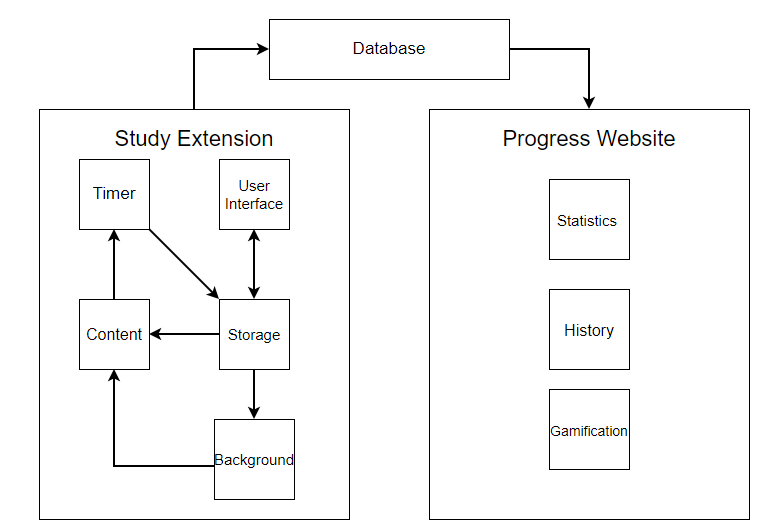
\includegraphics[width=15.0cm, height=10.0cm]{images/Design.png}
\end{figure}
\subsection{Module Descriptions}
\textbf{Study Extension:} A google chrome extension to help users focus on studying and remember to take breaks. Users have the option to log in which gives access to the website. The extension stores data about the study sessions in the database. \\\\
\textbf{User Interface:} The popup menu where users control the session, make choices about the timer, provide information, and can access the Progress Website.\\\\
\textbf{Storage:} Storage provided by the chrome.storage API that is shared among the scripts in the extension.\\\\
Background: Monitors the content pages to implement the whitelist and closes tabs that violate it. Continuously checks for mouse or keyboard inputs for statistics.\\\\
\textbf{Content:} Makes changes to the current tab's content such as running the Timer.\\\\
\textbf{Timer:} Displays a timer on the screen and counts down to the provided time. Contained and executed in the Content Script. Timer accesses storage when finished.\\\\
\textbf{Database:} Database that stores information about the study sessions such as total time studied and keyboard and mouse input frequencies. Verifies user login in the extension or the website before allowing access to the website information. \\\\
Progress Website: A locally hosted website which allows users to view information and progress on their study sessions. \\\\
\textbf{Statistics:} Displays information such as total time spent studying and input frequency. 
History: Displays information on previous sessions such as date, time began and ended, and total time studied for the session. \\\\
\textbf{Gamification:} Provides incentives for the users to study more through a game-like system where the total amount studied is translated to points and then to levels and titles.\\\\
\section{Implementation and Testing}
\subsection{Development environment and tools}
\subsection{Reused components}
\subsection{Testing scenarios and results}

% \section{References}

% \begingroup
% \renewcommand{\section}[2]{}
% \begin{thebibliography}{10}

%     \bigskip
% https://dev.to/penge/learn-the-most-useful-chrome-apis-by-creating-block-site-chrome-extension-2de8 

% \end{thebibliography}
% \endgroup


\end{document}
